\begin{center} 
\emph{``It's always good to take an orthogonal view of something. It develops ideas.'' -- Ken Thompson}
\end{center}

\section{Affine Transformations}\label{sec:isometry}
% \begin{Thm}[Cauchy-Schwarz Inequality] For all $\bb u, \bb v\in V$,
% \[ |\langle\bb u,\ \bb v\rangle| \le \Vert \bb u\Vert\Vert \bb v\Vert.\]
% \end{Thm}\vs
\begin{Thm}[Cauchy-Schwarz Inequality]\label{thm:CauchySchwarz} For all $\bb u, \bb v\in F^n$,
\[ |\bb u \cdot \bb v| \le \Vert \bb u\Vert\Vert \bb v\Vert.\]
\end{Thm}\vs

\begin{multicols}{2}
\begin{Thm}[The Triangle Inequality]\label{thm:triangleineq} For all $\bb u, \bb v\in F^n$, 
\[\Vert \bb u + \bb v\Vert  \le \Vert \bb u \Vert + \Vert \bb v\Vert.\]
\end{Thm}

\vfill
%\flushright
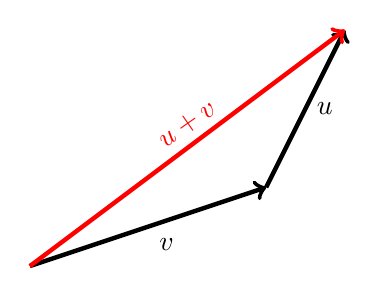
\begin{tikzpicture}
%\draw[dashed, ultra thick, gray] (1,2) -- (4,3);
%\draw[dashed, ultra thick, gray] (0,0) -- (1,2) ;
\draw[->, ultra thick] (0,0) -- (3,1) node[midway, below right] {$\bb v$};
\draw[->, ultra thick] (3,1) -- (4,3) node[midway, right] {$\bb u$};
\draw[->, ultra thick, red] (0,0) -- (4,3) node[midway, above, yshift = -5] {\rotatebox{35}{$\bb u + \bb v$}};
\end{tikzpicture}
\end{multicols}
\vs

\begin{Thm}[The Law of Cosines]\label{thm:lawcosines} Let $\bb u, \bb y\in F^n$. Then 
\[\bb u \cdot \bb y = \Vert \bb u\Vert\Vert \bb y \Vert \cos\theta,\footnotemark[2]\] where $\theta$ is the angle between the two line segments from the origin to the points identified with $\bb u$ and $\bb y$.
\end{Thm}\vs

\begin{Exam} Compute the angle $\theta$ between $\bb u = (6,-1)$ and $\bb v = (1,4)$ in $\R^2$.
\[\theta = \cos^{-1}\left(\dfrac{6(1)-1(4)}{\sqrt{6^2+(-1)^2}\sqrt{1^2+4^2}}\right) = \cos^{-1}\left(\dfrac{6-4}{\sqrt{36+1}\sqrt{1+16}}\right) =\cos^{-1}\left(\dfrac{2}{\sqrt{37}\sqrt{17}}\right) \approx \fbox{$85.43^\circ$}\qedhere\]
\end{Exam}\vs

From the previous theorem, if the angle between two vectors $\bb u$ and $\bb v$ is $90^\circ$, then the inner product $\bb u \cdot \bb v = 0$.\\

%In any inner product space $V$, the following two important inequalities hold.\\
%
%\begin{Def} Let $V$ be an inner product space. If $\bb u, \bb v\in V$, then we define the \textbf{angle} $\theta$ between $\bb u$ and $\bb v$ by the relation
%\[\theta = \cos^{-1}\left(\dfrac{\langle \bb u,\ \bb v\rangle}{\Vert\bb u\Vert \Vert\bb v \Vert}\right).\]
%\end{Def}\vs
%
%It then follows that 
%\[\langle \bb u,\ \bb v\rangle = \Vert\bb u\Vert\Vert \bb v\Vert \cos\theta.\footnote[2]{The reason for defining angles between vectors in this fashion is the law of cosines from trigonometry. In Euclidean space, the law of cosines gives 
%\[\Vert \bb u - \bb v\Vert^2 = \Vert \bb u\Vert^2 + \Vert \bb v\Vert^2 - 2\Vert \bb u\Vert\Vert \bb v\Vert\cos\theta.\] Thus, 
%\begin{eqnarray*}
%\Vert \bb u\Vert\Vert \bb v\Vert\cos\theta &=& \frac{1}{2}\left(\Vert \bb u\Vert^2 + \Vert \bb v\Vert^2 - \Vert \bb u - \bb v\Vert^2 \right)\\
%&=& \frac{1}{2}\left( u_1^2+\ldots + u_n^2 + v_1^2+\ldots+v_n^2 - (u_1-v_1)^2 - \ldots - (u_n-v_n)^2\right)\\
%&=& \frac{1}{2}\left(2u_1v_1 + \ldots + 2u_nv_n\right) = \bb u \cdot \bb v. 
%\end{eqnarray*} } \]
%
%\begin{Exam} Let $f(t) = 1-t^2$ and $g(t) = 2+t-t^2$ be polynomial in $\P_2$, whose inner product is determined by the values $t=-1,\ 0, 1$. Then the angle between $f$ and $g$ is determined as:
%\begin{eqnarray*}
%\theta &=& \cos^{-1}\left(\dfrac{f(-1)g(-1) + f(0)g(0) + f(1)g(1)}{\sqrt{f(-1)^2+f(0)^2+f(1)^2}\sqrt{g(-1)^2+g(0)^2+g(1)^2}}\right)\\
% &=& \cos^{-1}\left(\dfrac{0(0) + 1(2) + 0(2)}{\sqrt{0^2+1^2+0^2}\sqrt{0^2+2^2+2^2}}\right) = \cos^{-1}\left(\dfrac{1}{\sqrt{2}}\right) = \fbox{$45^\circ$}
%\end{eqnarray*}
%\end{Exam}

%\begin{Exam} Consider the inner product space $C[0,2\pi]$ with the integral inner product. Then 
%\[\langle \sin,\ \cos\rangle = \int_0^{2\pi} \sin(x)\cos(x)\dx = \dfrac{1}{2}\int_0^{2\pi} \sin(2x)\dx = -\dfrac{1}{4}\cos(2x)\bigg|_0^{2\pi} = 0.\] Therefore, $\sin \perp\cos$ in $C[0,2\pi]$.
%\end{Exam}\vs

\begin{Def}  A real square matrix $U$ is called \textbf{orthogonal} if $U^\top U = I$, that is, $U^{T} = U^{-1}$. A complex square matrix $U$ is said to be \textbf{unitary} if $U^* = U^{-1}$.
\end{Def}\vs

\begin{Thm} A square matrix $U$ is orthogonal (unitary) if and only if its column vectors form an orthonormal set.\end{Thm}\vs
%\begin{proof}
%Let $U$ be an $n\times n$ orthogonal matrix and let $\bb u_1, \bb u_2,\ldots, \bb u_n$ be the column vectors of $U$. Then
%\[U^\top U = \mtx{c}{\bb u_i}^\top\mtx{c}{\bb u_j} = \mtx{c}{\bb u_i^\top\bb u_j} = \mtx{c}{\bb u_i\cdot \bb u_j}.\] Therefore, $U^\top U = I_n$ if and only if $\bb u_i\cdot \bb u_j = \begin{cases} 0, & i\neq j\\ 1, & i=j\end{cases}$ if and only if the columns of $U$ are an orthonormal set.
%\end{proof}\vs

Since $U^\top = U^{-1}$ and $UU^\top = UU^{-1} = I$, it also follows that the row vectors of an orthogonal matrix $U$ must also form an orthonormal set.\\

Rotation and reflection matrices are examples of orthogonal matrices.\\

%Lay
\begin{Exam}\label{exam:1} The matrix 
\[U = \mtx{rrr}{3/\sqrt{11} & -1/\sqrt{6} & -1/\sqrt{66}\\ 1/\sqrt{11} & 2/\sqrt{6} & -4/\sqrt{66}  \\ 1/\sqrt{11} & 1/\sqrt{6} & 7/\sqrt{66}}\] is an orthogonal matrix. Note that 
\[U^\top U = \mtx{rrr}{3/\sqrt{11} & 1/\sqrt{11} & 1/\sqrt{11}\\ -1/\sqrt{6} & 2/\sqrt{6} & 1/\sqrt{6}  \\ -1/\sqrt{66} & -4/\sqrt{66} & 7/\sqrt{66}}\mtx{rrr}{3/\sqrt{11} & -1/\sqrt{6} & -1/\sqrt{66}\\ 1/\sqrt{11} & 2/\sqrt{6} & -4/\sqrt{66}  \\ 1/\sqrt{11} & 1/\sqrt{6} & 7/\sqrt{66}}\] \[= \mtx{ccc}{(9+1+1)/11 & (-3+2+1)/\sqrt{66} & (-3-4+7)/\sqrt{726} \\ (-3+2+1)/\sqrt{66} & (1+4+1)/6 & (1-8+7)/\sqrt{396} \\ (-3-4+7)/\sqrt{726} & (1-8+7)/\sqrt{396} & (1+16+49)/66} = I_3\qedhere\]
\end{Exam}\vs

\begin{Exam} Let $U = \mtx{cc}{ \frac{1}{2}(1+i) & \frac{1}{2}(1+i) \\ \frac{1}{2}(1-i) & \frac{1}{2}(-1+i)}$.  Note that 
\[UU^* = \mtx{cc}{ \frac{1}{2}(1+i) & \frac{1}{2}(1+i) \\ \frac{1}{2}(1-i) & \frac{1}{2}(-1+i)}\mtx{cc}{ \frac{1}{2}(1-i) & \frac{1}{2}(1+i) \\ \frac{1}{2}(1-i) & \frac{1}{2}(-1-i)} = \mtx{cc}{\frac{1}{2} + \frac{1}{2} & \frac{i}{2} - \frac{i}{2} \\ -\frac{i}{2} + \frac{i}{2} & \frac{1}{2} + \frac{1}{2}} = I_2\]
Therefore, $U$ is unitary.
\end{Exam}\vs

\begin{Thm} Let $U$ be an orthogonal (unitary) matrix, and let $\bb x, \bb y \in F^n$. Then \[(U\bb x)\cdot (U\bb y) = \bb x\cdot \bb y,\] that is, the matrix transformation $\bb x\mapsto \bb U\bb x$ preserves inner products.
\end{Thm}
\begin{proof}
\[(U\bb x)\cdot (U\bb y) = (U\bb x)^\top(U\bb y) =(\bb x^\top U^\top)(U\bb y)  = \bb x^\top(U^\top U)\bb y = \bb x^\top\bb y  = \bb x \cdot \bb y.\qedhere\]
\end{proof}\vs

Since multiplication by an orthogonal (unitary) matrix $U$ preserves inner products, as a consequence, it also preserves lengths, distances, angles, and orthogonality of vectors. For example, $\Vert U\bb x \Vert = \Vert \bb x\Vert$ and $\dist(U\bb x, U\bb y) = \dist(\bb x, \bb y)$ for any vectors $\bb x, \bb y$ and any orthogonal matrix $U$.\\

\begin{Thm} Let $\B$ and $\c$ be orthonormal bases of $F^n$. Then the change-of-basis matrix $\underset{\c \leftarrow \B}{\P}$ is orthogonal (unitary).
\end{Thm}\vs

\begin{Def} An \textbf{isometry} (or a \textbf{rigid motion}) is a function $R : F^n \to F^n$ such that $\dist(T(\bb x), T(\bb y)) = \dist(\bb x, \bb y)$ for all $\bb x, \bb y\in F^n$. \end{Def}\vs

Isometry, which translates as ``same-measure'' from Greek, are those maps that preserve distances and lengths. Using trigonometry, necessarily angles are preserved too. Therefore, an isometry is exactly a map which ``moves'' objects is the vector space without ``distorting'' them, that is, the image of a shape will be congruent to the original shape. Linear isometries are exactly multiplication by an orthogonal (unitary) matrix. \\

Orthogonal transformations are not the only way to make an isometry. Let $\bb b\in F^n$ be any vector in the vector space. We can define a transformation $T:F^n\to F^n$ by the rule $T(\bb x) = \bb x+\bb b$, called a \textbf{translation} by $\bb b$. If $\bb b\neq \bb 0$, then translation is not a linear map since $T(\bb 0) = \bb b \neq 0$. On the other hand, $\dist(T(\bb x), T(\bb y)) = \Vert (\bb x+\bb b) - (\bb y+\bb b)\Vert = \Vert \bb x+\bb b - \bb y-\bb b\Vert = \Vert \bb x - \bb y\Vert = \dist(\bb x, \bb y)$. If we allow for translations in a vector space, we must broaden our type of transformations to affine transformations.\\

\begin{Def} Let $T : F^n\to F^m$ be a function. We say that $T$ is an \textbf{affine transformation} if there exists a matrix $A\in F^{m\times n}$ and a vector $\bb b\in F^m$ such that $T(\bb x) = A\bb x+\bb b$ for all $\bb x\in F^n$.
\end{Def}\vs

Of course, a linear transformation is affine (when $\bb b=\bb 0$) and every translation is affine (when $A=I_n$). Affine transformations are very important in linear geometry. As translation maps are ALWAYS one-to-one (onto), an affine transformation $\bb x\mapsto A\bb x+\bb b$ is one-to-one (onto) if and only if the matrix transformation $\bb x\mapsto A\bb x$ is one-to-one (onto).\\

%NEW
\begin{Exam}\label{exam:affine} Consider the affine transformation $T : \R^3\to \R^3$ associated to the matrix $A = \mtx{rrr}{3&-1&1\\-3&2&0\\6&-3&2}$ and the translation vector $\bb b = (1, 2, 3)$. Then \[T\left(\vr{2\\0\\-1}\right) = \mtx{rrr}{3&-1&1\\-3&2&0\\6&-3&2}\vr{2\\0\\-1} + \vr{1\\2\\3} = \vr{5\\-6\\10} + \vr{1\\2\\3} = \vr{6\\-4\\13}.\]\vs

Is $\bb y = (2, -2, 4) \in \im(T)$? To answer this question, we solve the matrix equation $A\bb x + \bb b = \bb y\ \Rightarrow\ A\bb x = \bb y-\bb b = (1,-4,1)$:
\[\mtx{rrr|r}{3&-1&1&1\\-3&2&0&-4\\6&-3&2&1}\sim \mtx{rrr|r}{1&0&0&2\\0&1&0&1\\0&0&1&-4}.\] Therefore, $T(2,1,-4) = (2,-2,4)$.
\end{Exam}\vs

As mentioned above, an affine transformation $T:F^n\to F^n : T(\bb x) = A\bb x+\bb b$ cannot be linear if $\bb b\neq 0$ on $F^n$. On the other hand, we can realize affine transformations as matrix multiplication in a higher dimension. After all, $F^n$ is a naturally is a subset of $F^{n+1}$ and consists of all those vectors in $F^{n+1}$ whose last coordinate is zero. We may identify $F^n$ in $F^{n+1}$ with the hyperplane associated to the linear equation $x_{n+1}=1$. In other words, we will translate $F^n$ by the vector $\bb e_{n+1}$ and consider this $n$-flat. It will consist of all vectors in $F^{n+1}$ whose last coordinate is $1$. Suppose $\bb y = T(\bb x) = A\bb x+  \bb b$, which is the image of $\bb x$ under the affine transformation. Then 
\[\mtx{c|c}{A & \bb b \\ 0\ldots 0 & 1}\vr{\bb x\\ 1} = \mtx{c}{A\bb x+\bb b \\ 1} = \vr{\bb y\\1}.\] Hence, the affine transformation $T: F^n \to F^m$ can be extended to a linear transformation $L : F^{n+1} \to F^{m+1}$ in a higher dimension. \\

\begin{Exam} Using the affine transformation from \examref{exam:affine}, the standard matrix of the affine transformation is:
\[[T] = \mtx{rrr|r}{3&-1&1&1\\-3&2&0&2\\6&-3&2&3\\0&0&0&1}.\quad \text{Note that } T(2,0,-1) = \mtx{rrr|r}{3&-1&1&1\\-3&2&0&2\\6&-3&2&3\\0&0&0&1}\vr{2\\0\\-1\\1} = \vr{6\\-4\\13\\1}.\qedhere \]
\end{Exam}\vs

\begin{Thm}[Mazur-Ulam Theorem] If $T : F^n\to F^n$ is an isometry then, for all $\bb x\in F^n$, $T(\bb x) = U\bb x+\bb b$ for some translation vector $\bb b\in F^n$ and orthogonal (unitary) matrix $U \in F^{n\times n}$.
\end{Thm}\vs

Over $\R^2$ there are four types of isometries: rotation around a point in the plane, reflection across a line in the plane, translation, and glide reflection (the composition of a reflection and a translation, like footprints in the sand).

%%%%%%%%%%%%%%%%%% Exercises %%%%%%%%%%%%%%%%%%%
\startExercises{isometry}

\noindent For Exercises \ref{exer:findanglestart}-\ref{exer:findanglestop}, find the angle between the vectors $\bb u$ and $\bb v$ in $\R^n$.
\begin{enumerate}[!HW!, start=1,  label=$\spadesuit$ \arabic*., ref=\arabic*]
\begin{multicols}{3}
\item\label{exer:findanglestart} $\bb u = \vr{1\\1}$, $\bb v = \vr{3\\-1}$%%NEW
\itemspade $\bb u = \vr{1\\0\\-3}$, $\bb v = \vr{1\\2\\3}$%%NEW
\item\label{exer:findanglestop} $\bb u = \vr{1\\-1\\1\\1}$, $\bb v = \vr{1\\2\\3\\4}$%%NEW
\end{multicols}
\end{enumerate}

\noindent For Exercises \ref{exer:rigidstart}-\ref{exer:rigidstop}, identify whether of the transformation is an isometry. The graphic on the left will denote the original shape and the graphic on the right is the transformed shape.
\begin{enumerate}[!HW!, label=$\spadesuit$ \arabic*., ref=\arabic*]
\item\label{exer:rigidstart} The shape was translated and rotated.%%NEW
\begin{center}
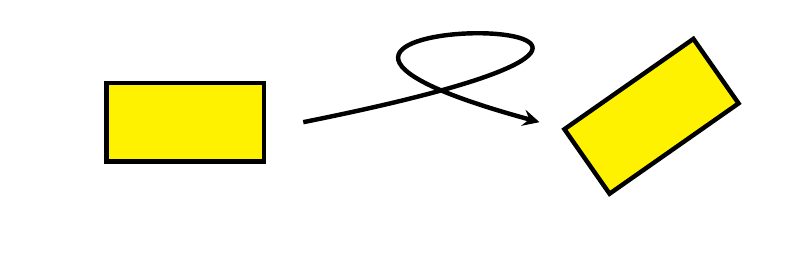
\begin{tikzpicture}
\clip (-1,-1) rectangle (8.5, 1.7);
\filldraw[ultra thick, fill=yellow] (0,0) rectangle (2,1);
\draw[ultra thick, -stealth] (2.5, 0.5) .. controls (10, 2) and (0, 2) ..  (5.5, 0.5);
\filldraw[ultra thick, fill=yellow, rotate=35, shift={(5,-4)}] (0,0) rectangle (2,1);
\end{tikzpicture}
\end{center}

\itemspade  The shape was translated and rotated.\footnotemark[8] 
\begin{center}
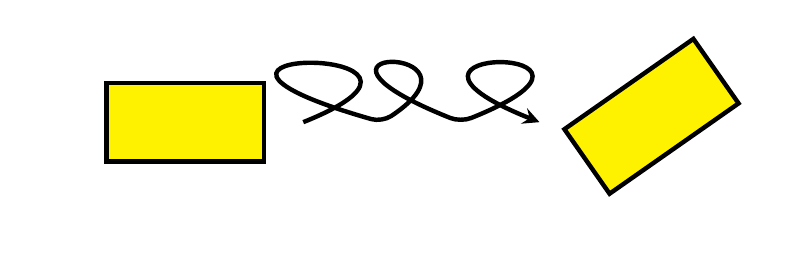
\begin{tikzpicture}
\clip (-1,-1) rectangle (8.5, 1.7);
\filldraw[ultra thick, fill=yellow] (0,0) rectangle (2,1);
\draw[ultra thick, -stealth, rounded corners] (2.5, 0.5) .. controls (5, 1.5) and (0, 1.5) ..  (3.5, 0.5) 
.. controls (5, 1.5) and (2, 1.5) ..  (4.5, 0.5) 
.. controls (7, 1.5) and (3, 1.5) ..  (5.5, 0.5);
\filldraw[ultra thick, fill=yellow, rotate=35, shift={(5,-4)}] (0,0) rectangle (2,1);
\end{tikzpicture}
\end{center}

\itemspade The shape was translated and increased in size.\footnotemark[3]
\begin{center}
\begin{tikzpicture}
\clip (-1,-1) rectangle (10.25, 1.7);
\filldraw[ultra thick, fill=yellow] (0,0) rectangle (2,1);
\filldraw[ultra thick] (2.5, 0.5) --  (5.25, 0.6) -- ($(5.25, 0.6)+(135:0.2)$) -- (5.6,0.5) -- ($(5.25, 0.4)+(-135:0.2)$) -- (5.25, 0.4) -- cycle;
\filldraw[ultra thick, fill=yellow, shift={(6,-0.6)}] (0,0) rectangle (4,2);
\end{tikzpicture}
\end{center}

\itemspade The object was translated and changed its shape from a rectangle to a circle, although the area stayed the same.
\begin{center}
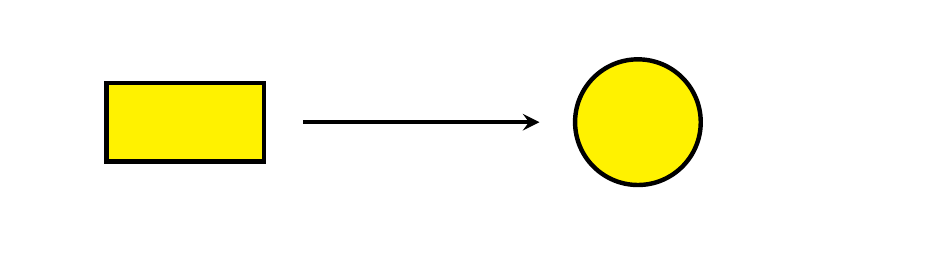
\begin{tikzpicture}
\clip (-1,-1) rectangle (10.25, 1.7);
\filldraw[ultra thick, fill=yellow] (0,0) rectangle (2,1);
\draw[ultra thick, -stealth] (2.5, 0.5) -- (5.5, 0.5);
\filldraw[ultra thick, fill=yellow, shift={(6.75,0.5)}] (0,0) circle (0.798);
\end{tikzpicture}
\end{center}

\itemspade The object was reflected.
\begin{center}
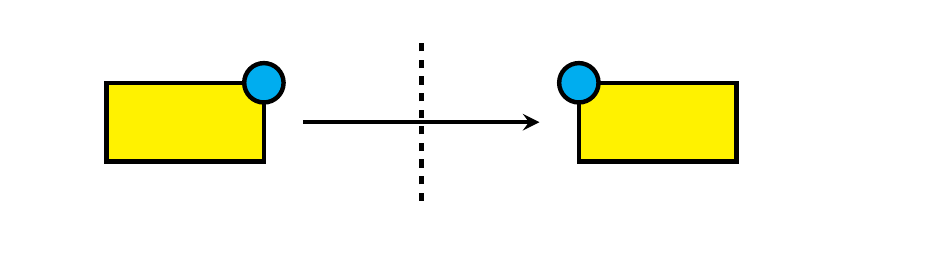
\begin{tikzpicture}
\clip (-1,-1) rectangle (10.25, 1.7);
\filldraw[ultra thick, fill=yellow] (0,0) rectangle (2,1);
\filldraw[ultra thick, fill=cyan] (2,1) circle (0.25); 
\draw[ultra thick, -stealth] (2.5, 0.5) -- (5.5, 0.5);
\draw[ultra thick, dashed] (4, -0.5) -- (4,1.5);
\filldraw[ultra thick, fill=yellow, shift={(6,0)}] (0,0) rectangle (2,1);
\filldraw[ultra thick, fill=cyan, shift={(4,0)}] (2,1) circle (0.25); 
\end{tikzpicture}
\end{center}

\itemspade In the following transformation, the shadow object denotes the original object and the opaque object denotes the transformed object.\footnotemark[9] 
\begin{center}
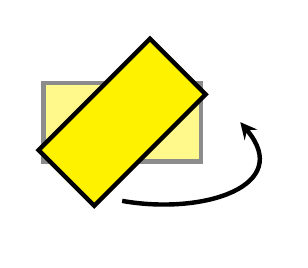
\begin{tikzpicture}
\clip (-0.2,-1) rectangle (3, 1.7);
\filldraw[ultra thick, fill=yellow!45!white, draw=black!45!white] (0,0) rectangle (2,1);
\draw[ultra thick] (1, -0.5) edge[-stealth, out=-10, in=-50, distance = 30, draw=black] (2.5, 0.5);
\filldraw[ultra thick, fill=yellow, rotate=45, shift={(-86:0.856)}] (0,0) rectangle (2,1);
\end{tikzpicture}
\end{center}

\itemspade The shape was translated and has been cut.
\begin{center}
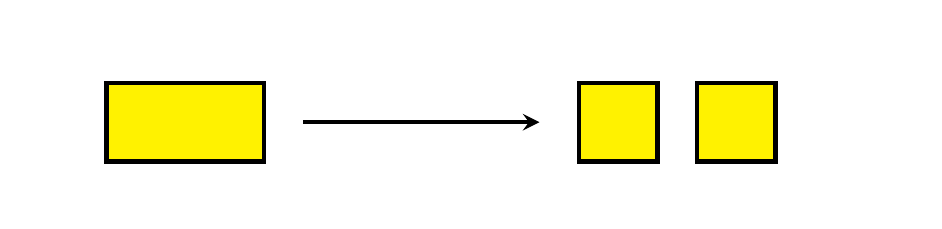
\begin{tikzpicture}
\clip (-1,-0.5) rectangle (10.25, 1.7);
\filldraw[ultra thick, fill=yellow] (0,0) rectangle (2,1);
\draw[ultra thick, -stealth] (2.5, 0.5) -- (5.5, 0.5);
\filldraw[ultra thick, fill=yellow, shift={(6,0)}] (0,0) rectangle (1,1) (1.5, 0) rectangle (2.5, 1);
\end{tikzpicture}
\end{center}

\item\label{exer:rigidstop} The following transformation is a little more difficult to visualize. Imagine the shape is transformed by placing it back exactly the way it was before, that is, the starting and stopping shape is identical. 
\begin{center}
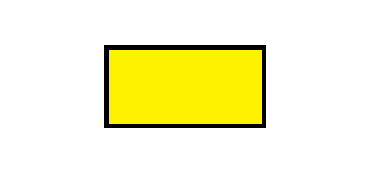
\begin{tikzpicture}
\clip (-1,-0.25) rectangle (3, 1.25);
\filldraw[ultra thick, fill=yellow] (0,0) rectangle (2,1);
\end{tikzpicture}
\end{center}
\end{enumerate}

\noindent For Exercises \ref{exer:translatestart}-\ref{exer:translatestop}, let $T : \R^2\to \R^2 : \bb x \mapsto \bb x+ \bb b$ be translation by $\bb b$, provided below. Let $P=\vr{2\\1}$.  Draw $P$ and $T(P)$ on the same gridlines.
\begin{enumerate}[!HW!, label=$\spadesuit$ \arabic*., ref=\arabic*]
\begin{multicols}{4}
\item\label{exer:translatestart} $\vr{1 \\ 0}$
\itemspade $\vr{0 \\-2}$
\itemspade $\vr{ -1\\-1}$
\item\label{exer:translatestop} $\vr{ -2\\1}$
\end{multicols}
\end{enumerate}

\noindent For Exercises \ref{exer:affinemapstart}-\ref{exer:affinemapstop}, consider the affine transformation $T : \R^3\to \R^3 : \bb x \mapsto A\bb x + \bb b$ associated to the matrix\\ $A = \mtx{rrr}{3&-1&1\\-3&2&0\\6&-3&2}$ and the translation vector $\bb b = \vr{1\\2\\3}$. 
\begin{enumerate}[!HW!]
\item\label{exer:affinemapstart} Compute $T(3,1,-5)$.
\item Find a vector $\bb x\in \R^3$ such that $T(\bb x) = (6,1,3)$. 
\item\label{exer:affinemapstop} Is $T$ one-to-one? Onto? Why or why not?
\end{enumerate}

\noindent For Exercises \ref{exer:affinetwomapstart}-\ref{exer:affinetwomapstop}, consider the affine transformation $T : \R^3\to \R^3 : \bb x \mapsto A\bb x + \bb b$ associated to the matrix\\ $A = \mtx{rrr}{1&0&-1\\2&2&2\\4&1&-3}$ and the translation vector $\bb b = \vr{-5\\6\\8}$. %Skyler Clark
\begin{enumerate}[!HW!, label=$\spadesuit$ \arabic*., ref=\arabic*]
\item\label{exer:affinetwomapstart} Compute $T(5,-2,4)$.
\itemspade Find a vector $\bb x\in \R^3$ such that $T(\bb x) = (-6,8,12)$. 
\item\label{exer:affinetwomapstop} Is $T$ one-to-one? Onto? Why or why not?
\end{enumerate}

%%%%%%%%%%%%%%%%%%% Footnotes %%%%%%%%%%%%%%%%%%%
 \mbox{}\vfill
 
\footnotetext[2]{For complex vectors, the real valued function $\cos : \R\to \R$ will need to be extended to the complex plane $\cos : \C\to \C$.}

\footnotetext[8]{Although the precious path of rotation and translation is different from the previous exercise, the starting and stopping positions of the shape are exactly the same. In this case, we say these two transformations \textbf{equal}. In particular, a transformation is determined by the image itself of the shape and not be the process which produces the image.}

\footnotetext[3]{This is an example of a \emph{dilation}. To shrink in size is called a \emph{contraction}.}

\footnotetext[9]{Notice that the center of the rectangle is not moved by the motion, that is, the transformation assigns this point to itself. We say that a point $P$ is a \emph{fixed point} if $P'=P$. The \emph{identity motion} is characterized as the transformation which assigns every point to itself, that is, all points are fixed. Can you find the identity motion in this homework set?}

\pagebreak